% $Date: 2024/06/04 17:45:48 $
% This template file is public domain.
%
% TUGboat class documentation is at:
%   texdoc tugboat
% or
%   https://texdoc.org/serve/tugboat/0
% or
%   https://mirrors.ctan.org/macros/\LaTeX\/contrib/tugboat/ltubguid.pdf

\documentclass{ltugboat}
\usepackage[T1]{fontenc}
\usepackage{graphicx}
\usepackage{microtype}
\usepackage[hidelinks]{hyperref}

\usepackage{tikz}
\usetikzlibrary{shapes}
\usepackage{standalone}

\title{Ximera: A \LaTeX{-}Based Open-Source Platform for Interactive
    Education}

% repeat info for each author; comment out items that don't apply.
\author{Jim Fowler}
\address{231 W. 18th Ave \\ Columbus, Ohio 43210 \\ USA}
\netaddress{fowler.291@osu.edu}
\personalURL{https://kisonecat.com/}
\author{Jason Nowell}
\address{1400 Stadium Rd \\ Gainesville, Florida 32611 \\ USA}
\netaddress{JNowell@ufl.edu}
\personalURL{https://www.jasonnowell.com/}
\author{Wim Obbels}
\address{Celestijnenlaan 200B \\ 3001 Leuven, \\ Belgium}
\netaddress{wim.obbels@kuleuven.be}
\personalURL{https://www.kuleuven.be/wieiswie/nl/person/00045050}
\author{Bart Snapp}
\address{231 W. 18th Ave \\ Columbus, Ohio 43210 \\ USA}
\netaddress{snapp.14@osu.edu}
\personalURL{https://people.math.osu.edu/snapp.14/}

%\ORCID{0}

% Please state if you'd like to receive a physical copy of the TUGboat
% issue or if electronic access suffices.  If you want a physical issue,
% please include the mailing address we should use, as a comment if
% you prefer it not be printed.

\begin{document}
\maketitle

\begin{abstract}
    TO WRITE
\end{abstract}

\section{Introduction}

Ximera is an open-source platform designed to create interactive online
educational
content using \LaTeX\ as the source code. Initially developed at the Ohio State
University, Ximera is now used by over a dozen institutions, including
the University of Florida and KU Leuven. By leveraging the semantic structure
of \LaTeX\ and integrating tools like Desmos, GeoGebra, and YouTube, Ximera
allows educators to generate high-quality \PDF\ print materials \emph{and}
interactive online content simultaneously from a single source.
\begin{center}
    \begin{tikzpicture}
        \node at (-1.8,.2)
        {\resizebox{.65cm}{!}{\documentclass[tikz]{standalone}
\begin{document}
\begin{tikzpicture}[rounded corners=.5pt]
\draw[fill=white] (0,0) -- (0,1.3) -- (.7,1.3) -- (1,1) -- (1,0) -- cycle;
\draw (.7,1.3) -- (.7,1) -- (1,1);
\end{tikzpicture}
\end{document}}};
        \node at (-1.8,.2) {\small \PDF};
        \node at (-2,0) {\resizebox{.65cm}{!}{\documentclass[tikz]{standalone}
\begin{document}
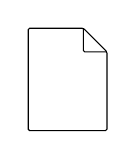
\begin{tikzpicture}[rounded corners=.5pt]
\draw[fill=white] (0,0) -- (0,1.3) -- (.7,1.3) -- (1,1) -- (1,0) -- cycle;
\draw (.7,1.3) -- (.7,1) -- (1,1);
\end{tikzpicture}
\end{document}}};
        \node at (-2,0) {\small \PDF};
        \node at (-2.2,-.2)
        {\resizebox{.65cm}{!}{\documentclass[tikz]{standalone}
\begin{document}
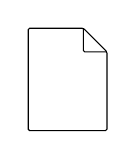
\begin{tikzpicture}[rounded corners=.5pt]
\draw[fill=white] (0,0) -- (0,1.3) -- (.7,1.3) -- (1,1) -- (1,0) -- cycle;
\draw (.7,1.3) -- (.7,1) -- (1,1);
\end{tikzpicture}
\end{document}}};
        \node at (-2.2,-.2) {\small \PDF};
        \draw[->] (-.6,0) -- (-1.4,0);
        \draw[->] (-.6,.2) -- (-1.4,.2);
        \draw[->] (-.6,-.2) -- (-1.4,-.2);
        \node at (0,0) {\resizebox{1cm}{!}{\documentclass[tikz]{standalone}
\begin{document}
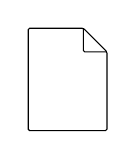
\begin{tikzpicture}[rounded corners=.5pt]
\draw[fill=white] (0,0) -- (0,1.3) -- (.7,1.3) -- (1,1) -- (1,0) -- cycle;
\draw (.7,1.3) -- (.7,1) -- (1,1);
\end{tikzpicture}
\end{document}}};
        \node at (0,0) {\LaTeX};
        \draw[->] (.6,0) -- (1.4,0);

        \node at (2,0) {\resizebox{1cm}{!}{\documentclass[tikz]{standalone}
\begin{document}
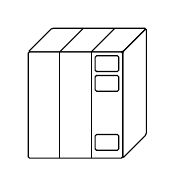
\begin{tikzpicture}[rounded corners=.5pt]
    \draw (0,0) rectangle (1.2,1.35);
    \draw (.4,0) -- (.4,1.35);
    \draw (.8,0) -- (.8,1.35);

    \draw (0,0)+(.85,1.1) rectangle ([shift={(.85, 1.1)}] .3, .2);
    \draw (0,0)+(.85,.85) rectangle ([shift={(.85, .85)}] .3, .2);
    \draw (0,0)+(.85,.1) rectangle ([shift={(.85, .1)}] .3, .2);

    \draw (1.2,0) -- (1.2,1.35) -- (1.5,1.65) -- (1.5,.3) -- cycle;

    \draw (0,1.35) -- (.3,1.65) -- (1.5,1.65) -- (1.2,1.35) -- cycle;
    \draw (.4,1.35) -- (.7,1.65);
    \draw (.8,1.35) -- (1.1,1.65);    
\end{tikzpicture}
\end{document}}};
        \draw[->] (2.6,0) -- (3.4,0);
        \node at (4,0) {\resizebox{1cm}{!}{\documentclass[tikz]{standalone}
\begin{document}
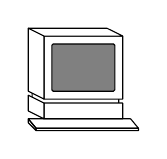
\begin{tikzpicture}[rounded corners=.1pt]
    \draw (-.15,-.1) rectangle (.95,.5);
    \draw[fill=white] (0,0) rectangle (1,.8);
    \draw[fill=white] (0,0) -- (-.2,.1) -- (-.2,.9) -- (.8,.9) -- (1,.8) -- (0,.8) --
    cycle;
    \draw (0,.8) -- (-.2,.9);
    \draw[fill=white] (0,-.05) -- (1,-.05) -- (1,-.25) -- (0,-.25) -- cycle;
    \draw[fill=white] (0,-.05) -- (0,-.25) -- (-.2,-.15) -- (-.2,.05) -- cycle;
    \draw[rounded corners=.5pt,fill=gray] (.1,.1) rectangle  (.9,.7);
    \draw (-.2,-.25) -- (1.1,-.25) -- (1.2,-.37) -- (-.1,-.37) -- cycle;
    \draw (-.2,-.25) -- (-.2,-.3) -- (-.1,-.4) -- (-.1,-.37) -- cycle;
    \draw (-.1,-.4) rectangle (1.2,-.37);
\end{tikzpicture}
\end{document}}};
        \node at (-2,-1) {Various};
        \node at (-2,-1.4) {\PDF s};
        \node at (0,-1) {Single};
        \node at (0,-1.4) {Source};
        \node at (2,-1) {Ximera};
        \node at (2,-1.4) {Server};
        \node at (4,-1) {Students};
        \node at (4,-1.4) {Engage};

    \end{tikzpicture}
\end{center}
To be clear, Ximera is designed to produce \emph{educational content}. Our
goals
are distinct from those of \TeX4ht and MathJax. While \TeX4ht seeks to
transform \LaTeX\ into \HTML, there is no additional interactivity. Moreover,
while \TeX4ht attempts to recreate the look of a \PDF\ online,
Ximera makes no such attempt to replicate a print-book experience. Ximera
instead attempts to do something reasonable
online, with the given semantic markup. To this end,
Ximera \emph{uses} \TeX4ht to convert a majority of the content to \HTML. In
turn,
\TeX4ht \emph{uses} MathJax to render mathematics online.

\section{Authoring Content in Ximera}

Ximera documents are written in \LaTeX. The \verb!ximera! document class
provides
additional commands supporting interactive online elements, such as answer
boxes,
multiple-choice questions, and other virtual manipulatives. Each document in
the \verb!ximera! document class corresponds to a single web-page, this pages
are ``glued'' together via a document using the \verb!xourse! document class.

Authors write the content on their own machines using their own tools, using
Docker, and git for version control.
This local setup allows authors to preview both \PDF\ and
\HTML\ outputs before publishing the content online.

\subsection{Document set-up}

Online content requires some organization and consistency that isn't required
with regular \LaTeX\
documents. Ximera courses are created with two \LaTeX\ documents, a
``main'' document of document class \verb!xourse! and all content documents,
which use document class \verb!ximera!. All Ximera files of either document
class \verb!ximera! or \verb!xourse! \emph{must} compile on their own for
successful deployment online. We give an example \verb!xourse! file below:
\begin{verbatim}[\small]
\documentclass{xourse}
\title{A Collection of Ximera Activities}
\begin{document}
\begin{abstract}
An example including activities in a Xourse.
\end{abstract}
\maketitle
\activity{aXimeraActivity.tex}
\activity{anotherActivity.tex}
\end{document}
\end{verbatim}
where each \verb!*.tex! file above is file of document class \verb!ximera! and
might look something like this:
\begin{verbatim}[\small] 
\documentclass{ximera}
\title{Some activity}
\begin{document}
\begin{abstract}
An example activity.
\end{abstract}
\maketitle
\begin{problem}
What is the answer to life, the universe, 
and everything?
\begin{solution}
\[
    \answer{42}
\]
\end{solution}
\end{problem}
\end{document}
\end{verbatim}

We can add functionality via user defined commands to the
document via a preamble, or macros document. Since every \verb!*.tex! file with
a \verb!\documentclass! must compile, the preamble file must be accessible  by
all files, with special attention paid to the directory paths.

For Ximera documents, the purpose of a preamble is to ensure \textbf{all files
    compile consistently. It is not for cosmetic changes.} Cosmetic changes to
Ximera environments may result in unpredictable behavior online.
With that said, Ximera provides several additional commands to help with the
construction of custom
\PDF s, with extensive cosmetic changes. They
\cs{pdfOnly}, \cs{prompt}, \cs{link}, \cs{activity}, \cs{practice},
\cs{sectionstyle},\cs{chapterstyle} and the environment \verb!onlineOnly!.
Typically authors create a second set of cosmetic macros that are loaded after
the preamble. This second set of macros, sometimes called ``printStyles''
redefines many commands. When inclosed in a \cs{pdfOnly} these commands have no
effect on online deployment.

\subsection{Special Ximera Commands and Environments}

The Ximera documentclass comes with many packages preloaded, including TikZ.

The documentclass also provides support for the following theorem-like
environments. We refer the reader to either the Ximera User Manual (Drafted at
the time of this writing) or to the Ximera~\LaTeX documentation.
% \verb!algorithm!, \verb!axiom!, \verb!claim!, \verb!conclusion!,
% \verb!condition!, \verb!conjecture!, \verb!corollary!, \verb!criterion!,
% \verb!definition!, \verb!example!, \verb!explanation!, \verb!exercise!,
% \verb!exploration!,
% \verb!fact!, \verb!formula!, \verb!hypothesis!, \verb!idea!, \verb!lemma!,
% \verb!model!,
% \verb!notation!, \verb!observation!, \verb!paradox!, \verb!proof!,
% \verb!problem!,
% \verb!procedure!,
% \verb!proposition!, \verb!question!, \verb!remark!, \verb!solution!,
% \verb!summary!, \verb!template!, \verb!theorem!, and \verb!warning!.
As of our current version, we cannot create new theorem-like environments to be
deployed online.

\subsection{Answer types}

Ximera provides several \LaTeX\ commands to create interactive elements within
documents, enhancing student engagement. These commands include:

\cs{answer}: Allows students to input answers directly in the online platform.
For example:

\begin{verbatim}[\small]
\begin{problem}
Differentiate $f(x) = x^2$.
\[
    \answer{2x}
\]
\end{problem}
\end{verbatim}

\verb|choice| environments: Used to create multiple-choice and “select all that
apply” questions, respectively. These questions can be graded automatically,
providing instant feedback to students.

\subsection{Graphics}

The preferred method of including graphics in a Ximera document is by using
TikZ. With that said, authors can also use \cs{includegraphics}. We advise
setting graphics paths in the preamble, so that all files can find them
regardless of their location in the file structure. Individual Ximera files as
well as Xourse files
must be able to load the graphics.

\subsection{Interactive Elements}

Ximera integrates with external tools like Desmos
and GeoGebra to create dynamic, interactive graphs that students can manipulate
in real time. Embedding a Desmos graph, for example, is as simple as:

\begin{verbatim}[\small]
\begin{center}
    \desmos{zwywds7med}{800}{600}
\end{center}
\end{verbatim}
Ximera also supports similar embeddings of YouTube videos, allowing educators
to integrate
multimedia resources into their lessons.

\subsection{Custom Validators}

Authors familier with JavaScript can use the environment \verb!javascript! to
create new ways of validating answers.
An example of this can be seen at:
\begin{center}
    https://xronos.clas.ufl.edu/mac1140exploreone/exploreFunctionsOne/explorePolynomials/Practice/factoringGeneral-Practice1
\end{center}

\subsection{Document Class Options}

By default, Ximera documents show all content. Alll, including answers and
instructor
notes. This is useful for authors during the development phase, as it ensures
they can review
the complete content. However, for classroom use, Ximera provides the handout
option, which suppresses answers and interactive elements, making it suitable
for distribution as student worksheets.

For example, the following document would display answers in development mode
but hide them when compiled with the handout option:
\begin{verbatim}[\small] 
\documentclass[handout]{ximera}
\begin{document}
\begin{problem}
What is the answer to life, the universe, 
and everything?
\begin{solution}
\[
    \answer{42}
\]
\end{solution}
\end{problem}
\end{document}
\end{verbatim}
This flexibility ensures that the same source document can be used for both
interactive online learning and traditional printed materials.

NOTE THE NESTING OF ENVIRONMENTS!

\section{Deploying Ximera content online}

Ximera relies heavily on Git for version control. We currently require that
content be hosted in a git repository for online deployment. In particular,
\emph{all source files must be commited to the git repository}.

\subsection{Docker and Visual Studio Code}

Our users are not programmers. With this in mind, we need a simple, consistent,
deploy process across all platforms. The Ximera developers mostly use Linux and
the initial
deployment tools were written
for Linux users. Supporting \macOS\ and Windows has been something of a
challenge. Our current strategy is to use Docker and VS Code to provide a
consistent build
environment for all users. Docker provides \emph{containers}, allowing users to
manage
dependencies and software versions consistently across platforms. VS Code has
good integration with Docker, and provides a \UNIX-like shell through
\emph{Windows Subsystem for Linux} (WSL).

Once Docker and VS Code are installed and set up, we provide a GitHub
repository
\begin{center}
    \url{https://github.com/ximeraProject/ximeraFirstSteps}
\end{center}
for testing of the set-up. Moreover within this this repository, VS Code
configuration files are found in \verb!.vscode! and Docker scripts are found in
!scripts!. When used with VS Code,

sers can interact with it through Visual Studio Code, using a built-in
terminal to execute commands for compiling and deploying Ximera documents.
Using Xake to ``Bake'' Ximera Documents

The Ximera build system, known as xake, automates the process of compiling
LATEX documents into both PDFs and interactive HTML files. The first time a
document is compiled, Xake downloads the required Docker containers and
processes the content. After the initial run, subsequent builds are much
faster, only compiling updated files.

To start the build process, users simply press the ``Bake'' button in Visual
Studio Code
After "baking" the content with Xake, the next step is to deploy the course
online. Ximera allows deployment to either a public server hosted by OSU or an
institution’s self-hosted server. To ensure security, Ximera requires users to
have GPG keys for authentication. These keys ensure that only authorized users
can deploy or update courses.

\section{Ongoing Development}

As of
the writing of this document, Ximera uses Docker containers to deploy with \TeX
Live 2019.
We are working (with the assistance of Michal Hoftich) to upgrade to a more
recent version of \TeX Live.
available for compiling documents and deploying them online.
is focused on two critical aspects
of Ximera: Streamlining the deployment process and expanding LTI 1.3
support.
We are leveraging Docker containers for deployment and designing an
assignment-grade database to seamlessly serve learners at institutions that
support LTI 1.3. Additionally, we are providing alternatives for
self-learners
and situations where LTI 1.3 support is not available.
\begin{center}
    \begin{tikzpicture}
        \node at (-3,1) [cloud, draw,cloud puffs=10,cloud puff arc=120,
            aspect=2, inner ysep=1em,scale=.8] {};
        \node at (-3,1) {LMS};
        \node at (-3,-1) {\resizebox{1cm}{!}{\documentclass[tikz]{standalone}
\begin{document}
\begin{tikzpicture}[rounded corners=.1pt]
    \draw (-.15,-.1) rectangle (.95,.5);
    \draw[fill=white] (0,0) rectangle (1,.8);
    \draw[fill=white] (0,0) -- (-.2,.1) -- (-.2,.9) -- (.8,.9) -- (1,.8) -- (0,.8) --
    cycle;
    \draw (0,.8) -- (-.2,.9);
    \draw[fill=white] (0,-.05) -- (1,-.05) -- (1,-.25) -- (0,-.25) -- cycle;
    \draw[fill=white] (0,-.05) -- (0,-.25) -- (-.2,-.15) -- (-.2,.05) -- cycle;
    \draw[rounded corners=.5pt,fill=gray] (.1,.1) rectangle  (.9,.7);
    \draw (-.2,-.25) -- (1.1,-.25) -- (1.2,-.37) -- (-.1,-.37) -- cycle;
    \draw (-.2,-.25) -- (-.2,-.3) -- (-.1,-.4) -- (-.1,-.37) -- cycle;
    \draw (-.1,-.4) rectangle (1.2,-.37);
\end{tikzpicture}
\end{document}}};
        \node at (-3,-2) {Students with LTI};
        \draw[->] (-3.1,-.4) -- (-3.1,.4);
        \draw[<-] (-2.9,-.4) -- (-2.9,.4);
        \node at (0,0) {\resizebox{1cm}{!}{\documentclass[tikz]{standalone}
\begin{document}
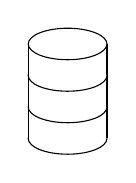
\begin{tikzpicture}[rounded corners=.5pt]
    \draw[fill=white] (.5,0) ellipse (.5cm and .2cm);  


    \draw[draw=none,fill=white] (0,0) rectangle (1,.4);
    \draw[] (0,0) -- (0,.4);
    \draw[] (1,0) -- (1,.4);    
    \draw[fill=white] (.5,.4) ellipse (.5cm and .2cm);  

    \draw[draw=none,fill=white] (0,.4) rectangle (1,.8);
    \draw[] (0,.4) -- (0,.8);
    \draw[] (1,.4) -- (1,.8);    
    \draw[fill=white] (.5,.8) ellipse (.5cm and .2cm);  


    \draw[draw=none,fill=white] (0,.8) rectangle (1,1.2);
    \draw[] (0,.8) -- (0,1.2);
    \draw[] (1,.8) -- (1,1.2);    
    \draw[fill=white] (.5,1.2) ellipse (.5cm and .2cm);  
\end{tikzpicture}
\end{document}}};
        \node at (0,-1) {Assignment};
        \node at (0,-1.4) {Database};
        \draw[->] (-2,.8) -- (-.6,.2);
        \draw[<-] (-2.1,.6) -- (-.7,0);
        \node at (3,-1) {\resizebox{1cm}{!}{\documentclass[tikz]{standalone}
\begin{document}
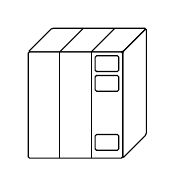
\begin{tikzpicture}[rounded corners=.5pt]
    \draw (0,0) rectangle (1.2,1.35);
    \draw (.4,0) -- (.4,1.35);
    \draw (.8,0) -- (.8,1.35);

    \draw (0,0)+(.85,1.1) rectangle ([shift={(.85, 1.1)}] .3, .2);
    \draw (0,0)+(.85,.85) rectangle ([shift={(.85, .85)}] .3, .2);
    \draw (0,0)+(.85,.1) rectangle ([shift={(.85, .1)}] .3, .2);

    \draw (1.2,0) -- (1.2,1.35) -- (1.5,1.65) -- (1.5,.3) -- cycle;

    \draw (0,1.35) -- (.3,1.65) -- (1.5,1.65) -- (1.2,1.35) -- cycle;
    \draw (.4,1.35) -- (.7,1.65);
    \draw (.8,1.35) -- (1.1,1.65);    
\end{tikzpicture}
\end{document}}};
        \node at (3,-2) {Ximera};
        \node at (3,-2.4) {Server};
        \node at (3,1) {\resizebox{1cm}{!}{\documentclass[tikz]{standalone}
\begin{document}
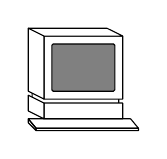
\begin{tikzpicture}[rounded corners=.1pt]
    \draw (-.15,-.1) rectangle (.95,.5);
    \draw[fill=white] (0,0) rectangle (1,.8);
    \draw[fill=white] (0,0) -- (-.2,.1) -- (-.2,.9) -- (.8,.9) -- (1,.8) -- (0,.8) --
    cycle;
    \draw (0,.8) -- (-.2,.9);
    \draw[fill=white] (0,-.05) -- (1,-.05) -- (1,-.25) -- (0,-.25) -- cycle;
    \draw[fill=white] (0,-.05) -- (0,-.25) -- (-.2,-.15) -- (-.2,.05) -- cycle;
    \draw[rounded corners=.5pt,fill=gray] (.1,.1) rectangle  (.9,.7);
    \draw (-.2,-.25) -- (1.1,-.25) -- (1.2,-.37) -- (-.1,-.37) -- cycle;
    \draw (-.2,-.25) -- (-.2,-.3) -- (-.1,-.4) -- (-.1,-.37) -- cycle;
    \draw (-.1,-.4) rectangle (1.2,-.37);
\end{tikzpicture}
\end{document}}};
        \node at (3,2) {Self-learner};
        \draw[->] (3.1,-.4) -- (3.1,.4);
        \draw[<-] (2.9,-.4) -- (2.9,.4);
        \draw[->] (2,.8) -- (.6,.2);
        \draw[<-] (2.1,.6) -- (.7,0);
        \draw[->] (2.3,-1) -- (.6,-.4);
        \draw[<-] (2.4,-.8) -- (.7,-.2);
    \end{tikzpicture}
\end{center}
BETTER DESCRIPTION

Ximera is constantly evolving. New features in development include a Docker
setup for easier deployment and a serverless option that enables document
compilation directly in the browser. The Ximera team is also working on
expanding gradebook functionality and adding more tutorials and examples to
help educators get started with the platform.

\bibliographystyle{tugboat} % tugboat's bibtex style
\nocite{book-minimal}	    % make the example bibliography non-empty
\bibliography{xampl}	    % xampl.bib comes with bibtex

\makesignature
\end{document}
